\section{Robot Dynamics and Control}
%
At issue in this chapter are the motions of various components of a robot given the forces, torques and momentum that act upon it. In rigid body dynamics, we typically represent these dynamics using nonlinear, second-order differential equations which are a function of the kinematics and kinetics of the robot.  While in principle, we can individually sum the forces and torques acting on an object, in practice, it is easier working with the system's \textit{Lagrangian, a summation of all the mechanical energies of the system}, as this tends to be less prone to error than summing together the Coriolis, centrifugal and inertial forces acting on the robot's links. 

The control problem for robot manipulators requires us knowing the dynamics of the robot. This is sometimes called the \textit{inverse dynamics problem} of a robot manipulator, \ie given the mass matrix, Coriolis forces and torques for all the individual robot joints, find the control law that yields a desired motion in space. Assuming that the model we have found is perfect, the control law is very simple. In practice, a feedback control (and sometimes coupled with a robust control) law needs to be derived to correct unmodeled uncertainties and improve trajectory following~\cite{Ogunmolu18IROS}.

There are two methods of controlling a rigid robot: \textit{joint space control} and \textit{workspace control}. In joint space control, a manipulation or navigation task is converted to a desired trajectory for the joints of a robot. We then find a control law to apply actuator torques to the joints of the robot in order to follow a given trajectory. In workspace control, the dynamics and control problem is changed into the task space of the robot so that trajectory commands are given in the coordinates of the end-effector.

\subsection{Lagrangian for Mechanical Systems }
%
For a system of $n$ particles obeying Newton's second law of motion, the time rate of change of the particle's momentum is the external force applied on the particle. Suppose $F_i$ is the applied force on the $i^{th}$ particle, $m_i$ is the particle's mass, and $r_i$ is the position, it follows from Newton's law that 
%
\begin{align}
	F_i = m_i r_i \quad r_i \in \bb{R}^3, i = 1, \ldots, n.
	\label{eq:RBD_Newton}
\end{align}
%
We are interested in the \cmt{material description} of the material where the overall degrees of freedom is constrained by the coupling between the individual robots. As such, we write out the constraints which govern the particle's positions as the following holonomic constraint\footnote{
%
If time enters the relation in the equation explicitly, then we have a rheonomic constraint, otherwise, the constraint is called sclerenomic constraint. A particle suspended from a tight rope in 3D space would be an example of a rheonomic constraint with the equation, $(x_1-1)^2  + (x_2 - b)^2 + (x_3-c)^2 - r^2 = 0$, while a particle on a carousel would be a sclerenomically-constrained system. Such a system would be described by the following equation, $x_1 = a \cos(\omega t + \phi); x_2 = a \sin (\omega t + \phi).$}. These are the constraints of position in a system.  
%
\begin{align}
g_i(r_1, \ldots, r_n) = 0, \quad j = 1, \ldots, k.
\label{eq:holonomic}
\end{align} 
%
In general, holonomic constraints are systems whose \dofs can be written in an algebraic relationship where the positions are a direct function of velocities. 

Constraints act on a system of particles through the application of \textit{constraint forces} such that they are forces that are normal to smooth surfaces in $\bb{R}^n$. Suppose we have the basis for the constraint forces (not necessarily orthonormal) as $\Gamma_1, \ldots, \Gamma_k \in \bb{R}^3n$ and $\lambda_j$ are the respective scaling factors for the $j^{th}$ basis elements, then we can write Newton's second law that governs the system of equations as 
%
\begin{align}
	F = \begin{bmatrix}
	m_1 \, I &  & 0 \\
	%
	& \ddots & \\
	%
	0 & & m_n \, I
	\end{bmatrix}
	%
	\begin{bmatrix}
	\ddot{r}_1  \\ \vdots \\ \ddot{r}_n
	\end{bmatrix} +  \sum_{j=1}^{k} \Gamma_j \lambda_j
\end{align}
%
where $\Gamma_j$ for the holonomic constraints of \eqref{eq:holonomic} can be taken as the gradients of $g_j$, essentially the level sets of $g_j(r) = 0$. 
%
While simple, this approach does not scale well to the configuration of the sort of rigid bodies we deal with in robotics. A better approach is to use a smaller set of variables that parameterizes the configuration of the system. For a system of $n$ particles with $k$ constraints, we find a set of $m = 3n − k$ variables $q_1, \ldots , q_m$ and smooth functions $f_1, \ldots, f_n$ such that 
%
\begin{align}
	r_i = f_i(q_1, \ldots, q_m), \quad i = 1, \ldots, n \\
	%
	g_j(r_1, \ldots, r_n) = 0, \quad j = 1, \ldots, k
\end{align}
%
where $q_i$'s are the generalized coordinates of the system, which in the case of robot manipulators is almost always the joint angles.  The forces expressed along the coordinates of the generalized coordinates of position are referred to as \textit{generalized forces}. 

\subsection{Euler-Lagrange Equations}
%
For a kinetic energy $T$ and a potential energy $V$, the \textit{Lagrangian, $L$}, of the system in generalized coordinates is the difference between the kinetic and potential energy, \ie
%
\begin{align}
L(q, \dot{q}) = T(q, \dot{q}) - V(q).
\label{eq:lagrange}
\end{align}
%
The equations of motion for a rigid body articulated system is of the form
%
\begin{align}
\dfrac{d}{dt}\dfrac{\partial L}{\partial \dot{q}_i} - \dfrac{\partial L}{\partial q_i} = \torque_i, \quad i = 1, \ldots, m
\label{eq:lagrange_compo}
\end{align}
%
where $\torque_i$ is the torque acting on the $i^{th}$ generalized coordinate. Written in matrix form equation, we can write the Euler-Lagrange equation of \eqref{eq:lagrange_compo} as
%
\begin{align}
\dfrac{d}{dt}\dfrac{\partial L}{\partial \dot{q}} - \dfrac{\partial L}{\partial q} = \torque.
\label{eq:lagrange_deri}
\end{align}
%
Equation \eqref{eq:lagrange_deri} is elegant because it reduces the number of coordinates we need to work with from $n$ to $m$ (the number of generalized coordinates) for a system. If there are no constraints to the system, then it follows that $n=m$. As such, we can choose $q$ to be the components of $r$, giving $T=\frac{1}{2}\sum m_i \|\ddot{r}_i^2\|$ so that \eqref{eq:lagrange_compo} reduces to \eqref{eq:RBD_Newton}.
%
Thus for a given robotic mechanical system, finding the dynamics is tantamount to deriving the kinetic and potential energies for the system based on that particular system characteristics. In the next two subsections, we will treat two examples -- a simple pendulum system and the dynamics of a mecanum wheel robot. 

\subsection{Dynamics of a spherical Pendulum}
%
We now consider the double pendulum of \autoref{fig:double-pendulum} with masses $m_1$ and $m_2$. We would like to find the overall torque of the system based on the Euler-Lagrange system of equations we just derived.
%
\begin{figure}[tb!]
	\centering
	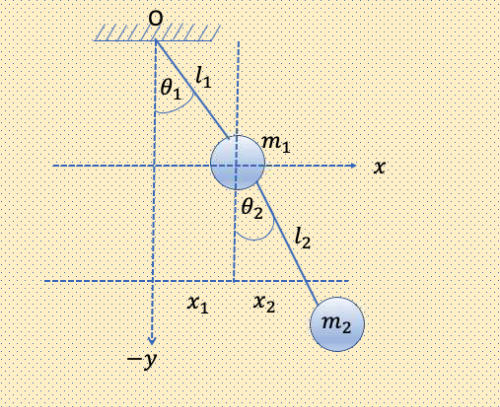
\includegraphics[width=.8\columnwidth]{figures/double-pendulum.png}
	\caption{The double pendulum with configuration is decribed by the angles $\theta_1$ and $\theta_2$.}
	\label{fig:double-pendulum}
\end{figure}
%
First, we write out the position vector of the masses as follows,
%
\begin{align}
	r(\theta_1, \theta_2) = \left(\begin{array}{c|c}
	l_1 \sin \theta_1 & l_1 \sin \theta_1  + l_2 \sin \theta_2
	\\
	-l_1 \cos \theta_1 & -l_1 \cos \theta_1  - l_2 \cos \theta_2
	\end{array}\right)
\end{align}
%
whose time derivative and second time derivative are respectively
%
\begin{align}
	\dot{r} = \left(\begin{array}{c|c}
	\dot{\theta}_1 l_1 \cos \theta_1 & \dot{\theta}_1 l_1 \cos \theta_1  + \dot{\theta}_2 l_2 \cos \theta_2
	\\
	\dot{\theta}_1 l_1 \sin \theta_1 & \dot{\theta}_1 l_1 \sin \theta_1  + \dot{\theta}_2 l_2 \sin \theta_2
	\end{array}\right)
\end{align}
%
and
%
\begin{align}
\ddot{r} = \left(\begin{array}{c|c}
\ddot{\theta}_1 l_1 \cos \theta_1 - \dot{\theta}_1^2 l_1 \sin \theta  & \ddot{\theta}_1 l_1 \cos \theta_1 - \dot{\theta}_1^2 l_1 \sin \theta  + \ddot{\theta}_2 l_2 \cos \theta_1 - \dot{\theta}_2^2 l_2 \sin \theta
\\
\ddot{\theta} l_1  \sin \theta_2 + \dot{\theta}_1^2 l_1 \cos \theta_1  & 
\dot{\theta}_1^2 l_1 \cos \theta_1  + \dot{\theta}_2^2 l_2 \cos \theta_2  + \ddot{\theta}l_1 \sin \theta_1 + \ddot{\theta}_2 l_2 \sin \theta_2 
\end{array}\right)
\end{align}
%
with the associated co-kinetic~\cite{Stramigioli2001} and potential energies
%
\begin{align}
	T = \frac{1}{2} m \|\dot{r}\|^2 = \frac{m_1}{2}l_1^2 \dot{\theta}_1^2 + \frac{m_2}{2}\left(l_1^2 \dot{\theta}_1^2 + l_2^2 \dot{\theta}_2^2 + 2 l_1 l_2 \dot{\theta}_1 \dot{\theta}_2 \cos(\theta_1 - \theta_2) \right)
\end{align}
%
and
%
\begin{align}
	V = g(m_1 \, y_1 + m_2\, y_2) = -m_1gl_1 \cos \theta_1 - m_2 g \left(l_1 \cos \theta_1 + l_2 \cos \theta_2\right)
\end{align}
%
where $g$ in this case denotes the gravitational acceleration.
%
We thus have the Lagrangian of the system as 
%
\begin{align}
	L & = T - V \nonumber \\
	  & = \frac{1}{2}(m_1 + m_2)l_1^2 \dot{\theta}_1^2 + \frac{1}{2}m_2 l_2^2 \dot{\theta}_2^2 + m_2l_1 l_2 \dot{\theta}_1 \dot{\theta}_2 \cos(\theta_1 - \theta_2) + (m_1 + m_2) g l_1 \cos \theta_1 + m_2 g l_2 \cos \theta_2 
\end{align}
%
Now writing the derivatives of the canonical momenta, we have
%
\begin{align}
\dfrac{d}{dt}\dfrac{\partial L}{\partial \dot{r}} &=  l_1^2(m_1+m_2) + m_2 l_2^2 \dot{\theta}_2 + m_2 l_1 l_2 \cos(\theta_1 - \theta_2)(\dot{\theta}_1 + \dot{\theta}_2) 
\end{align}
%
and we have for the associated generalized forces, 
%
\begin{align}
\dfrac{\partial L}{\partial r} =  %- m_2 l_1 l_2 \dot{\theta}_1 \dot{\theta}_2 \sin(\theta_1 - \theta_2)
  - (m_1 + m_2) g l_1 \sin \theta_1 - m_2 g l_2 \sin \theta_2
\end{align}
%
Thus, we have the system torque as 



\subsection{Dynamics of a Mecanum-Wheeled Robot}

\subsection{Robot Dynamics and the POE Formula}



